\newpage
\section{Демонстрация работы загрузчика}

Основываясь на предыдущем описании, сделаем не большой загрузчик, который должет поместиться в загрузочную область и выдать информацию о себе. В самом простом виде, он будет выглядить следующим образом.

\lstinputlisting[language=C++, caption={Исходный код простого загрузчика}]
{../../src/booter/mbr.c}

Но в таком виде код работать не будет, так как не учитываются следующие проблемы:
\begin{itemize}
\item pеальный режим работы процессора
\item elf файл
\end{itemize}

Решение в использовании специального шаблона для линкера

\lstinputlisting[language=C++, caption={Шаблон для линкера}]
{../../src/booter/linker.ld}

Собрасть получившийся код можно следующим образом

\begin{Verbatim}[frame=single]
$ gcc -c -g -Os -m32 -march=i686 -ffreestanding -Wall -Werror -I. -o mbr.o mbr.c
$ ld -static -melf\_i386 -Tlinker.ld -nostdlib --nmagic -o mbr.elf mbr.o
$ objcopy -O binary mbr.elf mbr.bin

$ dd if=/dev/zero of=floppy.img bs=1024 count=1440
$ dd if=mbr.bin of=floppy.img bs=1 count=512 conv=notrunc

$ qemu-system-i386 -fda floppy.img -boot a
\end{Verbatim}

Результат загрузки представлен на рисунке 1.

\begin{figure}[h!]
\centering
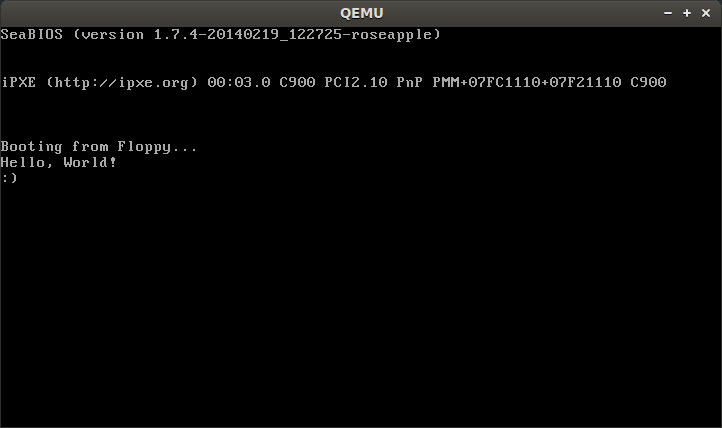
\includegraphics[scale=0.7]{res/qemu}
\caption{Запуск загрузчика}
\end{figure}